\documentclass{article}
\usepackage{tikz}
\usetikzlibrary[topaths]

\newcount\mycount
\newcount\endcount
\begin{document}
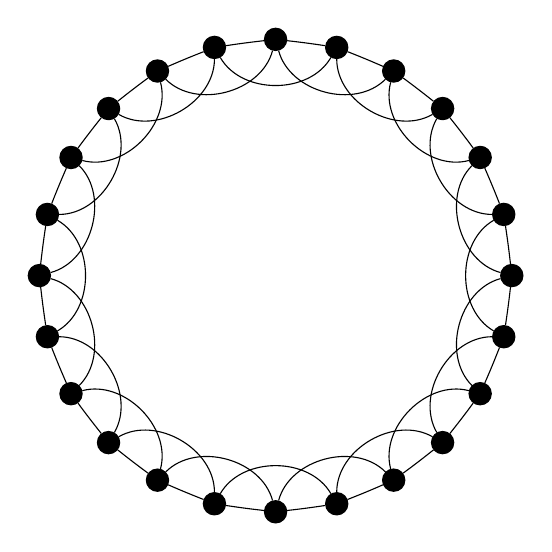
\begin{tikzpicture}
\foreach \number in {1,...,24}{
 \mycount=\number
 \advance\mycount by -1
 \multiply\mycount by 15
 \advance\mycount by 0
\node  [draw,circle,inner sep=0.1cm, fill=black] (N-\number) at (\the\mycount:3cm) {};
}
 \foreach \number in {1,...,22}{
        \mycount=\number
        \endcount=\mycount
        \advance\mycount by 1
        \advance\endcount by 2
        \path (N-\number) edge[bend right=1] (N-\the\mycount); %next neighbour, last 22-23 (line)
        \path (N-\number) edge[bend left, out=60, in=120] (N-\the\endcount); % next 2nd neighbour, 22-24 (arc)
  }
  \foreach \number in {23,...,24}{
  \mycount=\number
   \advance\mycount by -22
   \path (N-\number) edge[bend left, out=60, in=120] (N-\the\mycount); % 23 -1 and 24 -2
   }  
  \foreach \number in {23}{
  \mycount=\number
   \advance\mycount by 1
   \path (N-\number) edge[bend right=1] (N-\the\mycount); % 23 -24
   }
  \foreach \number in {24}{
  \mycount=\number
  \endcount=\mycount
   \advance\mycount by -23
   \path (N-\number) edge[bend right=1] (N-\the\mycount); % 24-1
   }
\end{tikzpicture}
\end{document}